% Documentation for University of Washington thesis LaTeX document class
% by Jim Fox
% fox@washington.edu
%
%    Revised for version 2014/11/13 of uwthesis.cls
%
%    This document is contained in a single file ONLY because
%    I wanted to be able to distribute it easily.  A real thesis ought
%    to be contained on many files (e.g., one for each chapter, at least).
%
%    To help you identify the files and sections in this large file
%    I use the string '==========' to identify new files.
%
%    To help you ignore the unusual things I do with this sample document
%    I try to use the notation
%       
%    % --- sample stuff only -----
%    special stuff for my document, but you don't need it in your thesis
%    % --- end-of-sample-stuff ---


%    Printed in twoside style now that that's allowed
%

\documentclass [12pt, proquest] {uwthesis}[2014/11/13]

%
% The following line would print the thesis in a postscript font 

% \usepackage{natbib}
% \def\bibpreamble{\protect\addcontentsline{toc}{chapter}{Bibliography}}

\setcounter{tocdepth}{1}  % Print the chapter and sections to the toc


% ==========   Local defs and mods
%

% --- sample stuff only -----
% These format the sample code in this document

\usepackage{alltt}  % 
\newenvironment{demo}
  {\begin{alltt}\leftskip3em
     \def\\{\ttfamily\char`\\}%
     \def\{{\ttfamily\char`\{}%
     \def\}{\ttfamily\char`\}}}
  {\end{alltt}}

% metafont font.  If logo not available, use the second form
%
% \font\mffont=logosl10 scaled\magstep1
\let\mffont=\sf
% --- end-of-sample-stuff ---




\begin{document}

%
% ==========   Preliminary pages
%
\prelimpages
%
% ----- copyright and title pages
%
\Title{Semantic Knowledge Management Framework\\for Learning Organizations}
\Author{Brendan Sweeney}
\Year{2015}
\Program{Cyber Security Engineering}

\Chair{Brent Lagesse}{Assistant Professor}{School of STEM Computing and Software Systems Division}
\Signature{Mark Kochanski}
\Signature{Marc Dupuis}
\Signature{Joe McCarthy}

\copyrightpage

\Degreetext{A report\\
            submitted in partial fulfillment of the\\
            requirements of the degree of}
\Degree{Master of Science in Cyber Security Engineering}
\textofCommittee{Project Committee:}

\titlepage

\setcounter{page}{-1}
\abstract{Knowledge management systems (KMS) allow organizations to capture, refine, and redistribute knowledge between members with minimal effort. Learning organizations, in particular, can benefit from such systems thanks to the capability these systems provide to transfer knowledge from individuals into a repository that is readily accessible to the entire group. While a complete knowledge management system incorporates a multitude of tools and resources, a major cornerstone of any modern KMS is a digital datastore in which information can be collected and correlated. In this project, Semantic Knowledge Management Framework, the author uses Semantic Web technologies to create a flexible foundation for the datastore component of a knowledge management system. This report begins with a brief comparison between relational database systems and graph-based information systems, including the author's reasons for choosing a graph-based approach built on RDF. Some similar applications are examined, both using relational databases and using Semantic Web frameworks. Next, some of the design decisions are discussed, along with the particular challenges of adapting programming objects to a dynamic RDF model and preparing SPARQL statements without a predefined schema. The project is demonstrated for use by a hypothetical computer security incident response team to track and manage assets, patches, policies, and team members. Finally, future goals and directions for the project are proposed.}

%
% ----- contents, etc.
%
\tableofcontents
\listoffigures
%\listoftables

%
% ----- glossary
%
\chapter*{Glossary}      % starred form omits the `chapter x'
\addcontentsline{toc}{chapter}{Glossary}
\thispagestyle{plain}

\begin{glossary}

\item[knowledge management] The practice of collecting, correlating, collating, and refining information so that it may be readily disseminated throughout an organization for members to act upon it.

\item[object] In RDF triples, the portion of the statement that provides the value that describes the subject.

\item[ORM] Object-RDF Model. Analogous to the object-relational model for relational databases, a description of how data modeled in the triplestore maps to the form and behavior of programming objects in running code.

\item[OWL] Web Ontology Language. A massive extension of RDF that includes finer classifications than RDFS and allows for logical inferences.

\item[predicate] In RDF triples, the portion of the statement that provides the property of the subject that is being described.

\item[RDF] Resource Description Framework. A cornerstone of the Semantic Web, RDF allows for uniquely identifiable (through URIs) resources to be describes in terms of triples which form a connected graph of semantically rich information.

\item[RDFS] Resource Description Framework Schema. An extension to RDF that provides additional pre-defined relationship types that can be used to describe resources.

\item[Semantic Web] A machine-readable representation of information on the World Wide Web that relates elements through semantic meaning.

\item[SKMF] Semantic Knowledge Management Framework; the software project that is discussed in this paper.

\item[SPARQL] SPARQL Protocol and RDF Query Language. Used to manipulate data stored in the RDF format.

\item[SPARQL endpoint] SPARQL Protocol and RDF Query Language. Used to manipulate data stored in the RDF format.

\item[subject] In RDF triples, the portion of the statement that identifies the resource that is being described.

\item[triple] In RDF, a three-part statement consisting of subject, predicate, and object. The subject is the resource being described, the predicate is a property of that resource, and the object is the value that applies to the given property of the given resource.

\item[triplestore] A datastore that is optimized for storage and retrieval of RDF triples.

\item[URI] Uniform Resource Identifier. In RDF, this is used to unambiguously identify a resource (subject or object) and a property (predicate).
 
\end{glossary}
 
%
% ----- acknowledgments
%
%\acknowledgments{% \vskip2pc
%  % {\narrower\noindent
%  The author wishes to express sincere appreciation to
%  University of Washington, where he has had the opportunity
%  to work with .
%  % \par}
%}

%
% ----- dedication
%
\dedication{\begin{center}in memory of my father, Dr. Frank Sweeney\end{center}}

%
% end of the preliminary pages


%
% ==========      Text pages
%
\textpages
\chapter{Introduction}
\label{intro}

Knowledge management -- the practice of capturing, refining, and redistributing knowledge -- is an important activity for any organization. It is of particular importance to organizations that operate with a high degree of knowledge transfer between employees; learning organizations. What sets knowledge management apart from information management is that information management is primarily concerned with maintaining the integrity and availability of an organization's information stores, while knowledge management is concerned with ensuring that information is actionable and useful to members of the organization
\cite{kmtoolkit}.
In order for that to happen, a mechanism must exist to allow for information to be refined, consolidated, correlated, and accurately retrieved. To that end, knowledge management systems (KMS) are designed to provide organizations with a centralized means to collect, refine, and redistribute knowledge between members. One important component of any modern KMS is a readily accessible digital datastore that allows members of an organization to contribute and refine information, then retrieve it based on some set of criteria, such as filters or keyword matches. The purpose of Semantic Knowledge Management Framework (SKMF) is to provide the means to construct such a datastore using Semantic Web technologies.


\section{The Semantic Web}
\label{intro:semantic}

The Semantic Web was proposed by Tim Burners-Lee in 1998
\cite{bernerslee}
as a means of opening up the Internet in a machine readable manner that allows simple Web services to locate and correlate information on behalf of users. The Semantic Web provides some technologies with novel characteristics for knowledge management. The two Semantic Web technologies used by SKMF are RDF to form information links and SPARQL
\cite{sparql}
to retrieve the information.


\subsection{RDF and Triplestores}
\label{intro:rdf}

Resource Description Framework
\cite{rdf}
(RDF) is the language that describes Semantic Web information. The smallest viable unit in RDF is the triple, a statement consisting of the uniform resource identifier (URI) of some resource, the URI of a specific property of that resource, and either a third URI or a literal value to provide meaning to the property. In RDF statements, these are referred to as the subject, predicate, and object, respectively. A collection of RDF statements provides a description of various resources and their relationships that can be represented as a directed graph, with subjects and objects as the nodes and predicates as the vertices directed from subjects to objects. While it is possible to serialize RDF statements into a form that is more compact than a complete list of triples, the information is typically kept in a triplestore that is further optimized for storage and retrieval of the statements, similar to a relational database system.

Relational database systems allow developers to define data models that map well to the objects in object-oriented programming. It is straightforward to assign each column from a table to an attribute of one programming object and define some predetermined behaviors to perform on those attributes. Due to its graph-based nature, RDF does not provide such a convenient mapping. In fact, the shape of the information changes as triples are inserted into and deleted from the triplestore. SKMF uses RDF, however, because the nature of information that will be placed in the system cannot be known beforehand. Any attempt by a developer to devise a schema of tables is merely a guess of what will be useful to the customer and in what way it will be useful. While very good guesses are possible, there will always missing attributes that the customer desires and extra attributes that the customer never uses, limiting how customers can represent their data. Despite its limitations, RDF is flexible enough to allow the customer define a personalized schema as information is added and forged into knowledge.


\section{Motivation for SKMF}
\label{intro:motive}

SKMF was originally conceived as a computer security incident response tool that would utilize Semantic Web linked data to build relationships between information assets, services, software, updates, vulnerabilities, patches, policy books, procedures, incident response team members, and other resources to aid incident responders in implementing security plans. Such a system would be able to pull information about vulnerabilities and patches from online sources of publication. It could be populated with asset information with the aid of a configuration management or network scanning tool that can identify networked resources. User information could be pulled from a network directory service or other source of team member information. Later, it was decided that the focus on incident response was not necessary and that a framework that would support quick deployment of such a system would be more useful. Thus, the focus of the project shifted to providing a general knowledge management platform that would allow users to define more specific uses of the application.

The intention of SKMF is to provide a linked data management interface that allows users to build custom ontologies and use those ontologies to describe sets of information. SKMF should provide a means of inputting information with guidelines for the user to make that information more useful. It should also provide an administrative interface for managing the users who are allowed to access and modify data, as well as restricting sets of data to certain users. It is not meant to convert an organization's existing information repositories into a linked data form. It is also not meant to provide end-to-end protection of transmitted information, as that falls largely on the Web server and triplestore used in the deployment environment. It is not meant to act as an inferencing engine for advanced ontologies, such as the Web Ontology Language
\cite{owl}
(OWL). Finally, it is not meant to describe a single knowledge domain, such as computer security incident response. Since incident response was the original inspiration for SKMF, however, this scenario is used in a mock case study of the application.

\chapter{Related Work}
 
The \TeX\ formatting program is the creation of
Donald Knuth of Stanford University.
It has been implemented on nearly every general purpose computer and
produces exactly the same copy on all machines.
 
\section{What is it; why is it spelled that way; 
and what do
really long section titles look like in the text and in the
Table of Contents?}
 
\TeX\ is a formatter.  A document's format is controlled
by commands embedded in the text.  
\LaTeX\ is a special version of \TeX---preloaded
with a voluminous set of macros that simplify most
formatting tasks.
 
\TeX\ uses {\it control sequences} to control
the formatting of a document.  These control sequences are usually
words or groups of letters prefaced with the backslash character
({\tt\char'134}).
For example,
Figure \ref{start-2} shows the text that printed the beginning
of this chapter.  Note the control sequence \verb"\chapter" that
instructed \TeX\ to start a new chapter, print the title, and
make an entry in the table of contents.  It is an example
of a macro defined by the \LaTeX\ macro package.
The control sequence \verb"\TeX", which prints the word \TeX,
is a standard macro from the {\it\TeX book}.
The short control sequence \verb"\\" in the title instructed \TeX\ to
break the title line at that point.
This capability is an example of an extension to \LaTeX\
provided by the uwthesis document class.
 
\begin{figure}
\begin{demo}
\singlespace
\\chapter\{A Brief\\\\Description of \\TeX\}

The \\TeX\\ formatting program is the creation of
Donald Knuth of Stanford University.
\end{demo}
\label{start-2}
\caption{The beginning of the Chapter II text}
\end{figure}
 
Most of the time \TeX\ is simply building paragraphs from
text in your source files.  No control sequences are involved.
New paragraphs are indicated by a blank line in the
input file.
Hyphenation is performed automatically.
 
\section{\TeX books}
 
The primary reference for \LaTeX\ is Lamport's second edition
of the \textit{\LaTeX\ User's Guide}\cite{Lbook}.
It is easily read and should be sufficient for thesis formatting.
See also the \textsl{\LaTeX\ Companion}\cite{companion} for descriptions
of many add-on macro packages.

Although unnecessary for thesis writers, the \textsl{\TeX book}
is the primary reference for \TeX sperts worldwide.
 
\section{Mathematics}
 
The thesis class does not expand on \TeX's
or \LaTeX's
comprehensive treatment of mathematical equation printing.%
\label{c2note}\footnote{%
% a long footnote indeed.
 Although many \TeX-formatted documents contain no
 mathematics except the page numbers, it seems appropriate
 that this paper, which is in some sense about \TeX,
 ought to demonstrate an equation or two.  Here then, is a statement 
 of the {\it Nonsense Theorem}.
 
 \smallskip
 \def\RR{{\cal R\kern-.15em R}}
 {\narrower\hangindent\parindent Assume a universe $E$ and a symmetric function
  $\$$ defined on $E$, such that for each $\$^{yy}$ there exists a
  $\$^{\overline{yy}}$, where $\$^{yy} = \$^{\overline{yy}}$.
  For each element $i$ of $E$ define
  ${\cal S}(i)=\sum_i \$^{yy}+\$^{\overline{yy}}+0$.
  Then if $\RR$ is that subset of $E$ where $1+1=3$,
  for each $i$
  $$\lim_{\$\to\infty}\int {\cal S}di =
      \cases{0,&if $i\not\in\RR$;\cr
             \infty,&if $i\in\RR$.\cr}$$
  \par}} % end of the footnote
%
The {\it\TeX book}\cite{book}, {\it \LaTeX\ User's Guide}\cite{Lbook},
and {\it The \LaTeX\ Companion}\cite{companion}
thoroughly cover this topic.
 
 
\section{Languages other than English}
 
Most \LaTeX\ implementations at the University are tailored
for the English language.  However, \LaTeX\ will format many
other languages.  Unfortunately, this author has never been successful in 
learning more than a smattering of anything other than English.
Consult your department or the Tex Users Group.
\smallskip
\begin{center}
{\tt http://tug.org/},
\end{center}
\smallskip
for assistance with non-English formatting.

Unusual characters can be defined via the
font maker \hbox{\mffont METAFONT} (documented by Knuth\cite{Metafont}).
The definitions are not trivial.
Students who attempt to print a thesis with
custom fonts may soon proclaim,
 
% Note.  This is not the ideal way to print Greek
\medskip
\begin{center}
``$\mathaccent"7027\alpha\pi o\kern1pt\theta\alpha\nu\epsilon\hat\iota\nu$
\ $\theta\acute\epsilon\lambda\omega$.''
 
\end{center}

\chapter{Architecture, Design, and Methods}
\label{method}

The code base of SKMF is written entirely in Python
\cite{python},
with Python 3.4 used as the active interpreter throughout development. This allows the code to be portable and forward-facing enough that it should be easily maintainable. The underlying architectural pattern used is model-view-controller (MVC). This pattern lends itself well to Web applications that utilize a backend datastore. Development followed the security development lifecycle (SDL) for Agile, as prescribed by Microsoft
\cite{secdevlifecycle}.
The Agile approach that was attempted is test-driven development (TDD), although project development veered heavily from this desired approach. For the most part, development stayed along the guidelines set out in the original project plan. Implementation details and justification for several design decisions are provided in the following sections.


\section{Developing With Modern Python}
\label{method:python}

Python was chosen as the development language for SKMF because the sole developer has some familiarity with Python development, the Python project has excellent documentation, and the Python interpreter makes Python applications highly portable. Python 3.4 was chosen as the target version because the widely deployed version 2.7 is no longer supported by upstream development and version 3.5, although currently considered stable, had not reached wide adoption at the time the SKMF project was started. As of this writing, version 3.4 is the stable version of Python on both Gentoo Linux, the primary environment of the developer, and Debian Linux, which has wide adoption amongst Linux users. Adhering to Python 3.4 compatibility ensures that the project can be easily maintained.

There are also some data structures that are particularly easy to work with in Python. Sets are useful when a collection should not contain any duplicates. They are especially useful when comparisons must be made between the contents of multiple collections, such as the intersection or the difference. Dictionaries, referred to in some other object-oriented programming languages as maps, are also quite versatile. The key needs to be a hashable datatype, but the value can be any Python object. This is convenient, for example, to hold a structure of RDF triples where the subject URI is the key and the rest of any triples pertaining to that subject are stored in another data structure as the value. Such a pattern is used extensively within SKMF, modeled after the Turtle serialization format for RDF and the JSON structure of SPARQL responses. Figure
\ref{skmf-triple}
shows this structure as a tree format.

\begin{figure}[h]
\singlespace
\begin{verbatim}
{<subject_uri>|<subject_label>:
    {`type': `uri'|`pfx'|`label',
     `value':
        {<predicate_uri>|<predicate_label>:
            {`type': `uri'|`pfx'|`label',
             `value':
                [{`type': `uri'|`pfx'|`label'|`literal',
                  `value': <object_uri>|<object_label>|<xml_literal>,
                  `xml:lang': <lang_string>,
                  `datatype': <xml_datatype>
                }]
            }
        }
    }
}
\end{verbatim}
\caption[Structure of a triple in SKMF]
 {\narrower The outer dictionary is keyed off of RDF subjects, identified by URI or label for query results. The corresponding value is a dictionary with only two entries: `type' to indicate the form of the subject and `value' to point to the rest of the triples, stored in another dictionary. This dictionary is similar in structure to the outer dictionary, only keyed off of RDF predicates. The inner dictionary for predicate values is similar to the one for subject values, except that the `value' key corresponds to a list of RDF objects stored as simple dictionaries. The object dictionary most closely matches the SPARQL query result specification, while the outer dictionaries extrapolate that form to resemble the more terse Turtle serialization style.
 }
\label{skmf-triple}
\end{figure}



\section{Semantic Model-View-Controller}
\label{method:mvc}

MVC is a popular architectural pattern when working with relational databases. Typically, a schema is developed in the database and some objects are designed around the schema to form the model. The view can be implemented with any interface that suits the necessary task, often some form of dynamic Web page rendering. This leaves the controller to perform all of the program logic and pass data between the model and the view. When a graph-based datastore with a dynamic schema is used instead, the problem requires a different approach
\cite{semanticwebprogram}.
Since the only two well-known object RDF model (ORM) modules for Python, RDFAlchemy
\cite{rdfalchemy}
and SuRF
\cite{surf},
are written for Python 2.7 and do not support Python 3, the object model for SKMF was implemented from scratch.


\subsection{Modeling Around RDF}
\label{method:orm}

When data are represented as a directed graph, as with RDF, it is possible for the model of the data to change as data are added and removed. This makes it difficult to maintain a schema and nearly impossible to enforce one. Two approaches are employed by SKMF to address this issue. First, a basic schema is hard-coded into the application to support some common RDF types and some features specific to the application. Second, the application utilizes parsers that allow users to define and extend virtually any custom schema.

A prime example of a hard-coded schema in SKMF is the `User' class. A user is treated like any other RDF resource, except that it is expected to have some known properties set and it may have other optional properties that get special treatment. One property that a user must have in the current version of SKMF is `skmf:hashpass', which is a salted hash of the user's password used for authentication. Note that in this notation `skmf:' is shorthand for the SKMF namespace, or the full URI where `hashpass' is defined. The only optional property of users that receives special treatment is `foaf:name', which is displayed in some parts of the Web interface. This is also an example of incorporating an external schema by using the `foaf' namespace
\cite{foaf}
instead of defining a custom property in the local namespace.

Custom schema generation is supported by the model code of SKMF. This is possible because of the generic manner in which resources are represented and the ability to limit SPARQL statements to specified named graphs. It would be possible, for instance, to define a schema using a collection of triples that describe how resources in that schema should behave, then place that collection in a named graph that is loaded by the controller component to be parsed for rendering appropriate forms for user interaction. The prototype user interface of SKMF does not, however, reveal this functionality to the user. Although, the Web interface does make use of a hidden schema to manage users and restrict user creation to an administrative user.

In order to better support system scaling, SKMF does not manipulate RDF directly. That task is left to a SPARQL endpoint, which is expected to be capable of handing the user's data storage needs. To speak with the SPARQL endpoint, queries are constructed from the aforementioned SKMF data structure for RDF triples, along with some extra information to help form and scope the query. SPARQL does not have the same concept of prepared statements as modern relational database systems, so queries are formed as string literals. This requires a number of parsers to generate different components of the query, depending upon the query type. For instance, a typical query statement first assembles the list of variable labels, then puts together the desired named graphs as a series of `FROM' statements, then forms the body of the query, which may require forming a set of `OPTIONAL' clauses that are used by SKMF to retrieve human readable labels whenever they are available. Finally, the processed segments are placed into a template for the appropriate query type, as depicted in Figure
\ref{sparql-template}.
Figure
\ref{sparql-statement}
illustrates a fully formed SPARQL statement.

\begin{figure}[ht]
\singlespace
\begin{verbatim}
{prefix}
SELECT DISTINCT {labels}
{graphs}
WHERE {{
  {body}
  {optional}
}}
\end{verbatim}
\caption[Template for SPARQL query statements]
 {\narrower This template outlines a general SPARQL query. `prefix' is replaced by the prefix lines from the active configuration. The other tags are replaced by generated string literals.
 }
\label{sparql-template}
\end{figure}

\begin{figure}[!ht]
\singlespace
\begin{verbatim}
PREFIX rdf: <http://www.w3.org/1999/02/22-rdf-syntax-ns#>
PREFIX rdfs: <http://www.w3.org/2000/01/rdf-schema#>
PREFIX xsd: <http://www.w3.org/2001/XMLSchema#>
PREFIX skmf: <http://example.com/skmf#>

    SELECT DISTINCT ?email ?person_label ?person ?email_label
    FROM <http://example.com/skmf>
    WHERE {
      skmf:www skmf:managedby ?person .
      ?person skmf:emailaddress ?email .
      OPTIONAL { ?email rdfs:label ?email_label . }
      OPTIONAL { ?person rdfs:label ?person_label . }
    }
\end{verbatim}
\caption[Generated SPARQL query statement]
 {\narrower SPARQL query statement formed by populating a template with values assembled by SKMF. This query asks for the person who manages the www resource and an email address. The `OPTIONAL' statements ask for human readable labels, if available.
 }
\label{sparql-statement}
\end{figure}


\subsection{Views and Control With Flask}
\label{method:flask}

Numerous Web frameworks are available for Python. The Flask framework
\cite{flask}
was selected for SKMF due to multiple factors. First, it is a full-stack Web framework that is modularized to avoid excessive overhead from unused functionality. Second, Flask more closely follows Python programming principles and better supports REST APIs than Django
\cite{django},
which is a very popular Web framework for Python. While SKMF is not specifically designed to be RESTful
\cite{restful},
it could be made to support a RESTful API at a later time. Third, Flask is available through a BSD license, making it more viable than a GPL-licensed framework for a project that may not be released under the same terms. Finally, Flask is extensively documented, even though some of the sanctioned modules are not.

The Web framework is relied upon to provide many of the security features desired of SKMF. Flask-WTF
\cite{flask-wtf}
automatically handles HTML filtering of input to mitigate cross-site scripting and it provides for use of synchronizer tokens to mitigate cross-set request forgery. Flask-Bcrypt
\cite{flask-bcrypt}
is used to generate a salted hash of user passwords that are stored in place of the plain text. Flask-Login
\cite{flask-login}
manages user sessions and authorization tokens, as well as providing a mechanism for directing unauthenticated users away from protected views. Flask does not, however, provide TLS support, so that must be implemented at deployment.


\section{Security Development Lifecycle in Agile}
\label{method:sdl}

Microsoft's SDL
\cite{secdevlifecycle}
prescribes an approach to software development that aids developers in identifying security and quality concerns throughout the development process. It is aimed primarily at larger development processes, but it includes recommendations for applying its key principles to an Agile development process. TDD was chosen as the Agile development approach for SKMF since the development team consisted of only a single member and since testability is one of the quality goals of SKMF. Unfortunately, it proved difficult to maintain TDD while working with Flask, so that approach primarily drove backend development.


\subsection{Identifying Security Issues in SKMF}
\label{method:threats}

One early step of the SDL is vulnerability analysis and threat modeling. The threat model for SKMF, shown in Figure
\ref{threat-model},
revealed that SKMF would have two main vectors of attack, under a certain set of assumptions. Due to its heavy reliance on the Python interpreter, it is assumed that the hosting system is running a patched version of Python with no untrusted or unmaintained modules. It is also assumed that unauthorized users cannot access the SKMF code directly. Under these assumptions, attacks may originate from the Web server or from the external SPARQL endpoint. Both of these systems are deemed to be outside of the control of SKMF.

\begin{figure}[p]
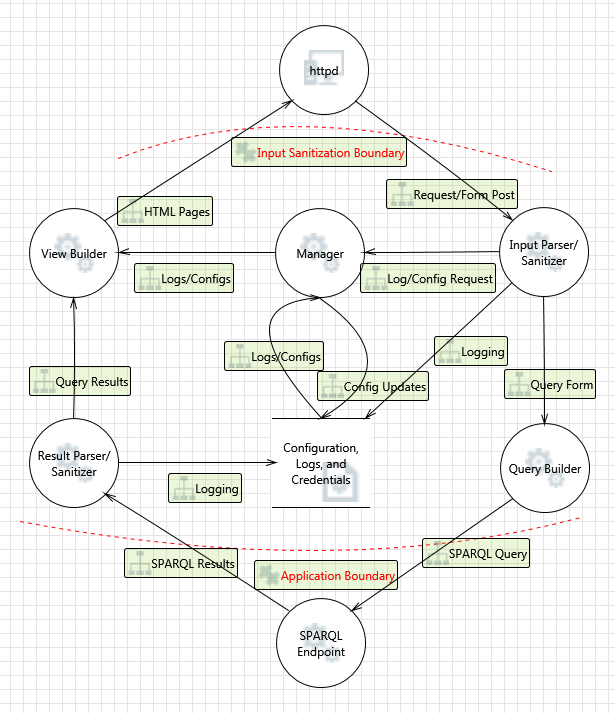
\includegraphics[width=6.5in]{threat-model}
\caption[Data flow diagram with threat boundaries]
 {\narrower Created with Microsoft Threat Modeling Tool 2016
  \cite{mstmt}.
  Data cross threat boundaries to and from the httpd Web server and the external SPARQL endpoint.
 }
\label{threat-model}
\end{figure}

Data from the Web server are considered untrusted because many of them are user supplied. The main threats identified by the model here are cross-site scripting (XSS), cross-site request forgery (CSRF), and information disclosure. An issue that was not identified by the modeling tool is injection. The first two issues are handled with Flask-WTF by always escaping text from form fields and by implementing synchronizer tokens. The third issue largely depends on secure deployment, with a secure connection between SKMF and the Web server and the use of TLS beyond that. The fourth issue requires that all input be handled safely and not passed directly to string parsers or SPARQL queries.

Steps taken within SKMF to mitigate information disclosure include handling user authentication with Flask-Login and providing the ability to scope queries and updates to specific named graphs. With a proper UI update, the use of these named graphs could allow an administrator to create a graph-based access control list for users, which could, itself, be stored in a restricted graph. Another measure to prevent information disclosure is the use of Flask-Bcrypt to provide a secure means of storing authentication tokens. Bcrypt mitigates brute-force attacks against password hashes by applying a salt to randomize the value that actually gets hashed and by using a hashing algorithm that is resource-intensive, making it very difficult to reverse. Use of a random salt also greatly reduces the likelihood that the hash of the password can be located within a rainbow table. Bcrypt does, however pose two problems for SKMF, since the hashing operations are performed on the server. The first problem is that the user's password is sent in clear text to the server. Even if it is encrypted through TLS, the clear text password is exposed for a brief time on the server and could be intercepted. The second problem is that the intensive nature of the hashing operation opens the server up to denial-of-service attacks should enough simultaneous logins be attempted. One possible solution to both problems is to offload the hashing operation onto the user's system, but that does not seem to be directly supported by Flask or any of the extensions currently used by SKMF.

Injection attacks can come in two forms. The first is format string injection, which occurs when a string formatting operation is performed directly on a user-supplied string that is assumed not to contain any string formatter tokens. The second is SPARQL injection, which occurs when a user-supplied string containing valid SPARQL escape sequences and syntax is sent to the SPARQL endpoint without being properly sanitized. Either injection attack could result in information disclosure or data corruption. To prevent format string injection, SKMF only applies the Python string format operation on static strings, like the template shown in Figure
\ref{sparql-template}.
In that template, the `body' and `optional' fields are both replaced by strings that may contain user input. That operation is performed by passing the replacement strings as arguments to the format() function, applied to the static template string. The replacement strings are constructed in a similar manner, with user input supplied as arguments to the format() function applied to some static string. Essentially, complex strings are constructed from the inside out and the format operation is only used on the outermost string at each layer, ensuring that it is never applied to a string that has been tainted by untrusted input.

SPARQL injection is more difficult to prevent. SPARQL does not offer prepared statements or parameterized queries, as do many SQL implementations, so input must be sanitized. Input sanitizing in SKMF is performed primarily by Flask-WTF, so HTML characters such as `\textless' and `\textgreater' should be escaped, making it difficult to construct a valid query injection. Since Flask-WTF handles any POST request, whether or not it was actually submitted through a Flask-WTF form, it should be difficult for an attacker to bypass the filters by crafting a special POST request. Also, SPARQLWrapper
\cite{sparqlwrapper},
which handles communication with the SPARQL endpoint, has strict requirements for how queries should be formed. SKMF forms queries as multi-line strings which means that any attempt to comment out the rest of a line during injection would most likely result in a query that SPARQLWrapper will reject. While these measures help to mitigate SPARQL injection attacks, further measures will need to be taken to properly safeguard SKMF. Ideally, a whitelisting approach will be taken when handling user input to ensure that any user-supplied field aligns with the SPARQL definition for a single variable, URI, or prefixed URI. This would ensure that only viable input could reach the SPARQL endpoint and it would provide an opportunity to alert users who have mistakenly provided invalid input.

Data from the SPARQL endpoint are considered untrusted because the security of the SPARQL endpoint is a matter of deployment. SKMF is likely to be deployed on the same host as the Web server with which it operates, but separation of duties would suggest that the datastore reside on a separate, more isolated host. This requires a secure, preferably encrypted connection between the hosts. It is, therefore, recommended that the SPARQL endpoint either support TLS or be accessible only over another secured transport, such as IPsec. The SPARQL endpoint also stores data provided by the user, which need to be retrieved. These data had to be sanitized by Flask-WTF before reaching the SPARQL endpoint, but it is still possible that something malicious is able to get through. SKMF does not, yet, sanitize outbound data.


\subsection{Attempted Test-Driven Development}
\label{method:tdd}

TDD worked well for the early model code. Simple test cases could be created and corresponding code written quite rapidly. Unfortunately, TDD did not work well for components that rely on Flask. Due to an initial lack of familiarity with the framework and, more specifically, testing within the framework, numerous difficulties were encountered when formulating test cases. Even test cases that appeared sound would frequently fail with Flask context errors. For the sake of making progress toward a functional prototype, TDD was abandoned for the duration of development.

SKMF was written with a bottom-up approach. The intention was to provide a solid foundation upon which a wide range of desired functionality could be built. It is possible, however, that a top-down approach would have worked better with TDD. In this approach, it would have been necessary to learn the proper testing procedures for Flask early on. The early test cases for validating the user facing components would then need only minor modification to verify proper support from the underlying elements that would be added later. This approach also would have ensured priority development of model code that is used by the prototype UI, allowing more time to implement demonstrable features.

\chapter{Results}
\label{result}

Semantic Knowledge Management Framework was developed with a focus on six quality goals. These goals are reliability, scalability, testability, maintainability, usability, and security. Progress was made, to some degree, in meeting each of the quality goals. Some of the goals, however, could not be thoroughly evaluated due to missing functionality or unavailable resources. None of them can be considered fully met in the current state of SKMF. What follows is a discussion of the different quality goals, the motivation behind them, the level of success in meeting them, and what is still required to properly fulfill them. The first three goals and their outcomes are discussed in the first section of this chapter. Each of the three remaining goals is discussed in a separate section.


\section{Unverified Quality Goals}
\label{result:unverified}

Any system that is part of vital business operations should be reliable and SKMF could find itself in that position. Reliability also supports availability, which is a tenet of good security. To support this goal, exceptions in SKMF are caught and reported without re-raising only at areas where program operation is not compromised by failure of the current operation. Also, consistency checks are made whenever an operation would alter data in the triplestore. There is, however, much still to do to ensure reliability. For one, extensive negative testing is required to ensure sane handling of unexpected inputs. Tests must also be performed in a multi-client setting to ensure that competing requests to not cause reliability issues. Only when SKMF can perform under duress for extended periods of time can this goal be considered achieved.

Scalability is another goal that is directed toward business environments. In order to scale to large, multisystem environments, SKMF utilizes a multi-threaded framework for handling Web content. It also separates itself from the Web server process and SPARQL endpoint so that these components may be implemented using something that suits the needs of the organization. Unfortunately, there are some serious shortcomings in the prototype implementation of SKMF. While the Web framework uses multi-threading, SKMF does not make use of threads for backend operations. A bigger issue with scaling comes from a lack of caching, which results in excessive queries to the SPARQL endpoint. This problem would be particularly detrimental in a multi-user environment with frequent system accesses. A final improvement to support scalability is to offload some tasks, most notably password hashing, onto the client. Again, failure to do this would have greater consequences in a multi-user environment. Once these measures are taken, satisfactory scalability could be considered achieved once SKMF is capable of processing requests on par with the Web server behind which it operates.

Since SKMF initially followed test-driven development, the goal of testability naturally fit the project. As the project moved away from TDD, however, this goal increasingly waned. The result is a split between testable code and poorly tested code. Test cases exist for all of the model components of SKMF. While not exhaustive, they demonstrate how easily test cases for those components can be written. The view and controller components, on the other hand, have only minimal test cases. The code in these components is also of considerably lower quality than that written for the model, so it is likely more difficult to test. Therefore, to achieve testability, the view and controller code should be cleaned up to better match the model code and proper Flask testing should be used on those components.


\section{Maintainability}
\label{result:maintain}

Maintainability is a personal goal for SKMF. The project may be shelved for some time, then picked up again at some point in the future. It may also be shared or even open-sourced, giving new developers the opportunity to build upon it. In either case, the code should be accessible and understandable to future developers. The interface needs to be clear enough others to use without touching the code, as well. Also, developers should not have to worry about breaking the code in unexpected ways when making modifications. Several steps were taken to ensure the various facets of this goal.

Simplicity promotes maintainability. Whenever possible, Python built-in data structures provide the underlying functionality. This minimizes custom logic and provides developers with familiar constructs. Complex layouts of the data structures follow similar patterns wherever they appear, providing consistency. Documentation accompanies every module, every class, and the vast majority of functions, methods, and attributes. SKMF lacks direct support for internationalization, but consideration of this issue resulted in the migration of most textual output into an English localization file, providing for simpler implementation of i18n at a future time. Templates contain HTML comments to mark their points of entry and exit, which aids in tracking the origin of content in Web views. SKMF avoids the use of deprecated classes and methods, with great care taken to ensure the absence of deprecation warnings from testing branches, where applicable. Finally, SKMF avoids long import chains to minimize coupling. With all of these practices in place, SKMF achieves its highest level of quality in maintainability.

There is still room for improvement. Better separation of concerns between the model and the controller would present more intuitive interfaces. View code requires pruning, modularization, and simplification. There is also an open question of whether to keep the innermost dictionary for SKMF triples modeled after the JSON response for SPARQL queries, keeping those structures directly compatible; or to model them after the outer dictionaries, which would allow all levels of the triples to be handled in a uniform manner, even recursively, if so desired. Naming conventions, while mostly consistent, could use some disambiguation. More improvements may be recognized as more eyes review the code.


\section{Usability}
\label{result:usability}

For a project designed to simplify the user experience when handling semantic data, usability is extremely important. While knowledge management systems, in general, support collection and retrieval of knowledge, SKMF seeks to present users with an intuitive method of interacting with the links that represent such knowledge. Essentially, users should be able to add information to the system with enough detail to easily identify and describe it, create meaningful connections between the new information and the information that already exists in the system, and easily derive meaning from the connections and relationships identified through intuitive queries. Such meaningful user interaction creates the core value for a semantic knowledge management system.

SKMF makes several assumptions on behalf of the user. For one, users tend to prefer simple, natural language labels to complex URIs. Queries, therefore, automatically append optional clauses for these labels, which appear in the user interface wherever the requested resource displays. Also, when new information is added, users are required to provide some, preferably meaningful, descriptions before submitting the form. Another assumption is that users want links to information sources. So, when a textual label for a resource is rendered, it renders as a hyperlink to a page that fully describes that resource, in case the query that retrieved that resource did not retrieve all of the desired connections thereto. An example of the resulting Web page is shown in Figure
\ref{info-page}.
Users are assumed, as well, to be unfamiliar with RDF. To aid these users, SKMF populates dropdown lists with elements categorized by where they are most likely to appear in a triple, with classes separated from properties. An example is shown in Figure
\ref{resource-page}.

\begin{figure}[!ht]
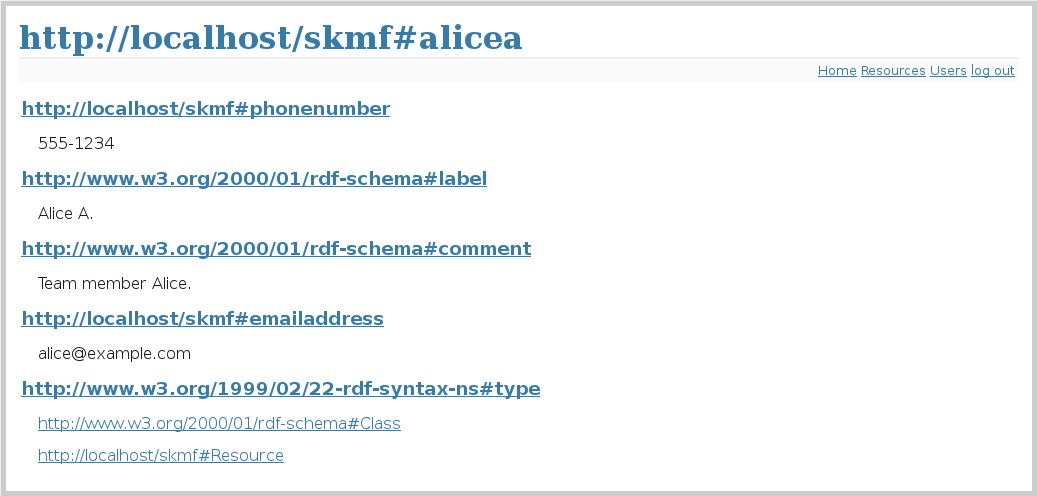
\includegraphics[width=6.5in]{info-page}
\caption[Resource information page of SKMF]
 {\narrower All information about Alice A. in SKMF.
 }
\label{info-page}
\end{figure}

\begin{figure}[!ht]
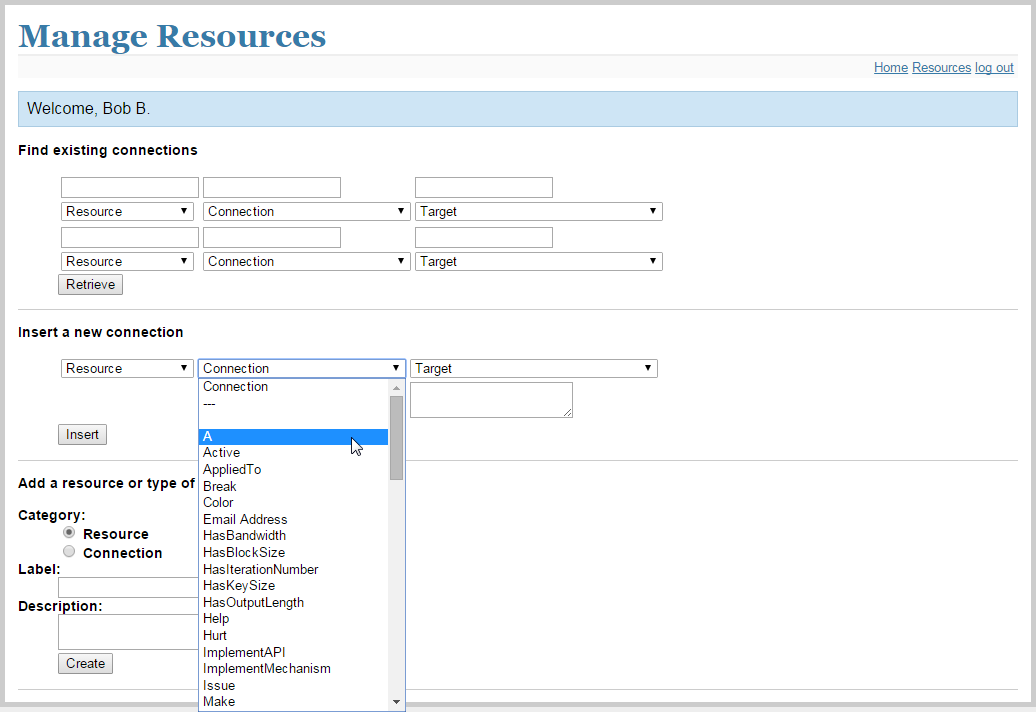
\includegraphics[width=6.5in]{resource-page}
\caption[Resource management page of SKMF]
 {\narrower Web page for managing resources in SKMF. The top form allows for a SPARQL query to be constructed with two sets of constraints. Text fields allow input of variables and dropdowns allow for selection of existing URIs, represented by their labels. The middle form allows for descriptions to be added to an existing resource. The bottom form allows for the addition of a new resource, with the `Label' and `Description' fields both required. A non-default selection from a dropdown always overrides the contents of a text field.
 }
\label{resource-page}
\end{figure}

Unsurprisingly, the usability goals proved overly ambitious for the scope of this project, so the prototype falls short on numerous points. The type of meaningful user interaction desired for SKMF requires implementation of dynamic Web pages with forms that grow in size to support arbitrary levels of refinement. There was insufficient time during this project for the necessary techniques to be learned and implemented. While the code is thoroughly documented, the UI lacks helpful documentation. In addition, a mock case study, discussed in the next section, revealed that some of the assumptions, as they are currently handled, hinder the user experience. For instance, the treatment of resources added to the system becomes awkward when that resource is a person, as many of the attributes one normally associates with people are not immediately available in the forms. Also, the controller automatically appends a language tag to string literals as they are added to help support future internationalization, as discussed in section
\ref{result:maintain}
on maintainability. This places a needless language restriction on numeric strings, such as phone numbers. As the user interface is refined, the basic assumptions require refinement, as well, driven by feedback from potential users.

Aside from a dynamic overhaul of the UI, usability in SKMF would benefit from various backend improvements. Just as textual labels are requested for resources, full descriptions could be requested, as well, and made available to the frontend to use, for instance, in tooltips. Form text could be parsed to determine its purpose, which would allow savvy users to craft more complex queries than the system allows through selections. Subtle exposure of SPARQL functions and their use in the controller would also allow for richer user interaction. A seed ontology would aid the system in performing such actions intelligently. User experience is one area of software development wherein improvements can always be made and SKMF has a lot of potential for growth and experimentation in this area.


\subsection{Mock Case Study}
\label{result:case-study}

In lieu of a full case study, SKMF was partially validated through a mock case study involving only the developer. For that exercise, the STAC
\cite{ontosec}
was imported into SKMF. Outside of SKMF, a short list was made of physical servers, software, team members, known vulnerabilities, and mitigations. In addition, a set of tasks were defined, such as locating servers that were susceptible to certain vulnerabilities and retrieving the contact information of the person responsible for maintaining them. The developer then used SKMF to enter the information from the list and create connections, such as who was responsible for which servers and which vulnerabilities applied to which software packages. Finally, the developer attempted to execute the tasks with a minimal number of steps.

Although it lacked the insight that would have been gained from exposure to outside parties, the mock case study did reveal many of the usability issued found with SKMF. For one, the STAC ontology was not immediately recognized by SKMF because of its reliance on OWL, so support had to be added in code instead of through the user interface. Also, team members could not be assigned names, as are users when they are added to the system, because only the administrative user management interface has access to the `foaf' namespace where many person-centric properties are readily available. The need for proper prompts and help text was also made apparent, as the queries used to fulfill the tasks mostly relied on knowledge SPARQL syntax and likely would not have been constructed properly through the forms by a user who is unfamiliar with SPARQL.

Aside from the shortcoming, the mock case study did validate some of the potential uses for SKMF. Adding resources and applying properties proved to be straightforward. Also, obtaining enough information from a query to follow a link for more information was simple enough to make browsing a viable way to locate information in small datasets. Most importantly, it was demonstrated that queries can return the sort of indirect relationship that SKMF is meant to provide. For instance, one task was to retrieve the phone numbers of the people responsible for any servers affected by a specific vulnerability. By supplying the vulnerability, some specific relationships, and a couple of variables, it was possible to bring up a list of the responsible parties which contained links to their full information, including phone numbers. While this task took two steps in the SKMF prototype interface, it could realistically be reduced to a single step with a more dynamic interface that provides useful prompts to the user.


\section{Security}
\label{result:security}

Since SKMF was developed under the Cyber Security Engineering program at the University of Washington, Bothell, security is an obvious quality goal for the project. Security also serves a practical purpose for an application that is accessible over a network and used to manage sensitive information. Such an application must provide confidentiality, integrity, and availability by enforcing authentication, authorization, and non-repudiation
\cite{incidentresponse}.
Whether an action performed against the system is malicious or unintentionally detrimental, it should not result in violation of the aforementioned tenets within the system, requiring the system to handle these actions in a secure manner. The following sections discuss what threats face a system like SKMF, what safeguards are currently implemented in SKMF to mitigate those threats, and what safeguards should be implemented to provide better mitigation.


\subsection{Ensuring Confidentiality}
\label{result:confidentiality}

A breach of confidentiality in SKMF primarily means disclosure of information from the triplestore to an unauthorized party, as this is the sole repository for information. Interception of a user's credentials is a breach of confidentiality that could lead to spoofing and a larger breach. Such attacks could be made between SKMF and the SPARQL endpoint, between SKMF and the Web server process, or between the Web server and the user. Spoofing attacks are particularly potent because they permit an attacker to bypass most safeguards with little effort.

Data passing between SKMF and the Web server is managed primarily by Flask. So long as Flask communicates with the Web server in a sane manner, transactions should occur sanely, as well. Therefore, SKMF comes with a strong recommendation to deploy it on the same host as the Web server to minimize the opportunity for eavesdropping. It is also recommended that the Web server be configured with TLS, as this is beyond the control of SKMF. Similarly, since SKMF uses pure SPARQL to communicate with the widest possible range of SPARQL endpoints, security between the two is largely a matter of deployment. The triplestore should not be deployed on the same host as the Web server, as this increases the attack surface on a key data asset. Even on an intranet, the triplestore is best deployed on a separate host from SKMF, as SKMF communicates directly with the Web server and may introduce vulnerabilities to the triplestore. SPARQLWrapper, which SKMF uses to connect with the SPARQL endpoint, supports TLS, so it is recommended to pair the triplestore with a SPARQL endpoint that supports TLS. If this is not an option, then a secure tunneling protocol, such as IPsec, should protect the connection.

Flask-Login provides the authentication resources used to govern access to the system. In addition, SKMF counters spoofing by supporting graph-based access controls. Sensitive data may reside in a named graph that is inaccessible to unprivileged users. An example of this is the `user' graph, which is only accessible to the administrative user. By segregating data into graphs, administrators minimize the impact of compromised user credentials. As with any networked system, the administrative credentials are highly sensitive and should be properly safeguarded. The full support for graph-based access control is not exposed in the Web interface, so this needs to be implemented before this feature can adequately protect a deployment.


\subsection{Ensuring Integrity}
\label{result:integrity}

The biggest integrity concern in SKMF is the state of the triplestore. The information retrieved therefrom should accurately reflect the information written thereto. Information in transit also requires integrity, particularly if it results in modification of the triplestore. Loss of integrity may result from malicious tampering or from failure to validate information passed between processes. The latter is easier to protect against within SKMF, as it likely produces detectable defects in the data. Tamper protection requires proactive mitigation.

Many of the safeguards that ensure confidentiality also provide integrity checks. TLS and IPsec both use cryptographic message authentication codes to verify that data were not altered in transit. Most triplestores automatically verify data integrity to prevent corruption. While SKMF does not implement tamper protection, it does provide checks to deter unintended alteration of information. Whenever the user creates a new resource, the triplestore is checked for the existence of a resource that already meets the provided description and, if found, loads that resource instead of creating it anew, alerting the user to the existence of the resource, as well. When updates are performed on a resource, they are first checked against the existing information about that resource to avoid collisions. The sane portions of the update are then applied and their description returned to the user, allowing the user to take appropriate action if the returned description differs from the desired update.

One way to greatly improve checks for inadvertent modification in SKMF would be to provide a description of the changes back to the user and request confirmation before committing them. This may pose a usability issue, though, so it may work best to allow the users to set an option that enables or disables this feature, with an administrative option to override any user's selection. Integrity maintenance could also be improved by coding strict checks for adherence to the RDF and SPARQL specifications into the controller of SKMF to make intelligent decisions about how to treat all data that are destined for the SPARQL endpoint.


\subsection{Ensuring Availability}
\label{result:availability}

If SKMF is not available to legitimate users, then it only serves to consume resources that are better allocated elsewhere. While many aspects of availability depend upon the deployment environment, there are others for which SKMF holds sole responsibility. A process crash would render the system inaccessible until the process could be restarted. Excessive query requests could result in unacceptably slow response times and traffic congestion. It is even possible to cause SKMF to consume excessive processing power by flooding it with login attempts for a legitimate user with the wrong password, since the hashing operation to verify the password is performed on the server. There are other ways to reduce available, but this sampling represent the biggest threats to SKMF.

The prototype of SKMF lacks robust availability assurance. It catches known exceptions during procedures that are not crucial to continuing operation, but there are still procedures that can cause a crash, which an attacker may be able to exploit. Improved error handling would greatly mitigate this vulnerability. Excessive queries currently pose a real threat. As briefly mentioned in section
\ref{result:unverified}
concerning scalability, queries are not cached and performance suffers even with small datasets. A more intelligent query system and a caching mechanism would mitigate attacks involving query floods while providing increased performance to the user. Another issue mentioned with scalability is performing password hashing on the server. The Bcrypt algorithm is used for hashing because it is designed to be slow and requires significant resources to reproduce a hash. To prevent an attacker from abusing this to consume excessing processing power, the hashing operating could be delegated to the client. This would have the added benefit of preventing plain text passwords from crossing the network, reducing the opportunity for interception of credentials and spoofing of users.

\chapter{Conclusion}

There is still much to be done.

\printendnotes

%
% ==========   Bibliography
%
%\nocite{*}   % include everything in the uwthesis.bib file
\bibliographystyle{plain}
\bibliography{sweeney-mscse2015}

%
% ==========   Appendices
%
\appendix
\raggedbottom\sloppy
 
% ========== Appendix A
 
\chapter{Where to find the files}
 
The uwthesis class file, {\tt uwthesis.cls}, contains the parameter settings,
macro definitions, and other \TeX nical commands which
allow \LaTeX\ to format a thesis.  
The source to
the document you are reading, {\tt uwthesis.tex},
contains many formatting examples
which you may find useful.
The bibliography database, {\tt uwthesis.bib}, contains instructions
to BibTeX to create and format the bibliography.
You can find the latest of these files on:

\begin{itemize}
\item My page.
\begin{description}
\item[] \verb%http://staff.washington.edu/fox/tex/uwthesis.html%
\end{description}

\item CTAN
\begin{description}
\item[]  \verb%http://tug.ctan.org/tex-archive/macros/latex/contrib/uwthesis/%
\item[]  (not always as up-to-date as my site)
\end{description}

\end{itemize}

\vita{Brendan Sweeney is a graduate student in the Cyber Security Engineering program at the University of Washington, Bothell campus. With considerable luck, he will be the first official graduate of this program since its inception in Fall, 2013.
}


\end{document}
